\section{Tablero y Conexionado}
\frame{
	\ifdebug
	\frametitle{Outline\hfill{\color{red} \emph{F}}}
	\else
	\frametitle{Outline}
	\fi
	\tableofcontents[currentsection]
	}

\subsection*{Generalidades}
% Una subsection* crea un nuevo "grupo de puntos"

\frame{
	\ifdebug
	\frametitle{Generalidades\hfill{\color{red} \emph{F}}}
	\else
	\frametitle{Generalidades}
	\fi

	\begin{columns}
		\begin{column}{0.55\textwidth}
		{\color{newcolor}Objetivos:}
		\begin{itemize}
		 \item \textbf{Alimentar} los elementos de la planta
		 \item \textbf{Encender} motores
		 \item \textbf{Adquisición} de variables
		 \item \textbf{Control} de la válvula
		 \item \textbf{Seguridad}
		\end{itemize}
		
		\vspace{.5cm}
		{\color{newcolor}Distinguimos:}
		\begin{itemize}
		 \item Cableado de potencia
		 \item Cableado de señal
		\end{itemize}


		\end{column}
		\begin{column}{0.45\textwidth}
			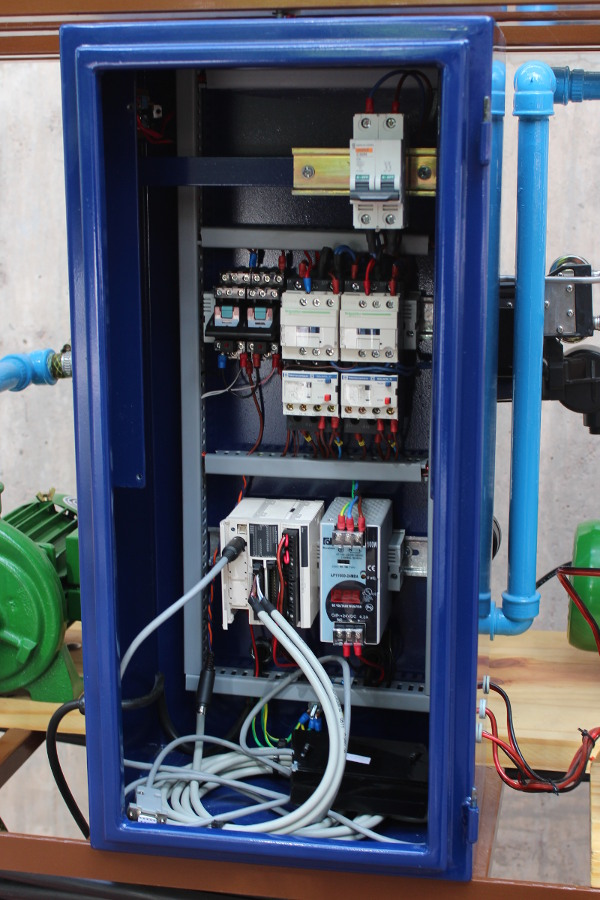
\includegraphics[width=\textwidth]
{Sections/3-Tablero/Images/IMG_5097.JPG}
		\end{column}
	\end{columns}
}

\subsection*{Cableado de potencia}
\frame{
	\ifdebug
	\frametitle{Cableado de potencia\hfill{\color{red} \emph{F}}}
	\else
	\frametitle{Cableado de potencia}
	\fi

	
	Elementos eléctricos, destinados a \textbf{alimentar} los motores de 
las bombas y los circuitos lógicos

	\vspace{-.25cm}
	\begin{columns}
	 \begin{column}{.45\textwidth}
	\begin{itemize}
	 \item \textbf{Interruptor termomagnético}
	 \item \textbf{Fuente de alimentación} $24\,V$ - $100\,W$
	 \item \textbf{Alimentación de motores}
	 \end{itemize}
	 \end{column}
	 
	 \begin{column}{.55\textwidth}
	 \begin{center}
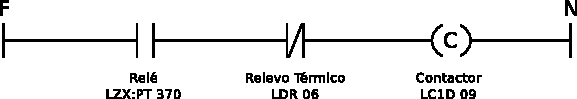
\includegraphics[width=\textwidth]{Sections/3-Tablero/Images/ladderConexion.pdf}

\vspace{.5cm}

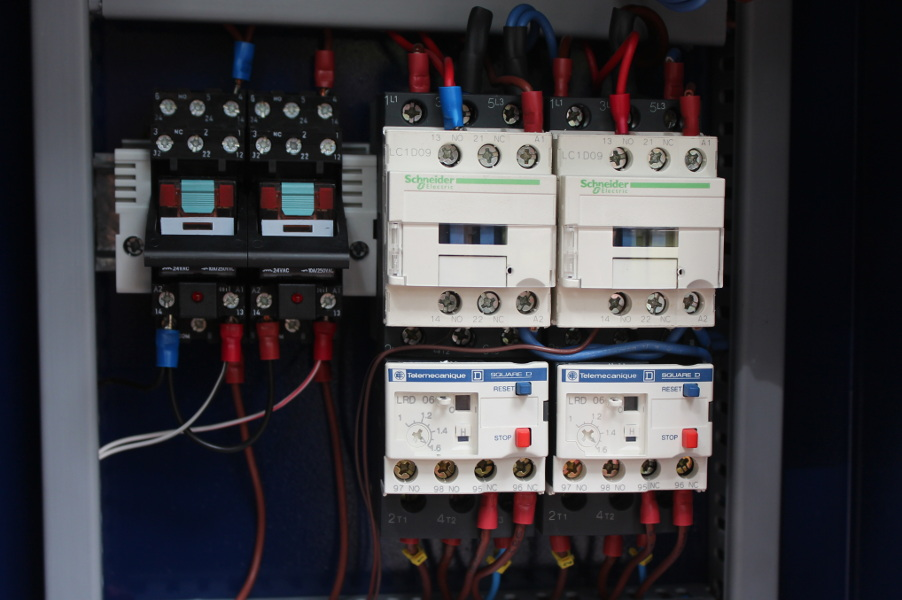
\includegraphics[width=\textwidth]{Sections/3-Tablero/Images/IMG_5093.JPG}

	\footnotesize
	Detalle alimentación de motores
	 \end{center}
	\end{column}
\end{columns}
}

\subsection*{Cableado de señal}
\frame{
	\ifdebug
	\frametitle{Cableado de señal: PLC\hfill{\color{red} \emph{F}}}
	\else
	\frametitle{Cableado de señal: PLC}
	\fi

	\textbf{Controlador Lógico Programable}
	
	\vspace{.25cm}
	\begin{columns}[t]
		\begin{column}{0.45\textwidth}
			
			\begin{itemize}
			 \item Procesador - memoria
			 \item I/O discretas
			 \begin{itemize}
			  \item Activación de motores 
			  
			  \texttt{Q0.0} - \texttt{Q0.1}
			  \item Enclavamientos 
			  
			  \texttt{I0.0} - \texttt{I0.1}
			 \end{itemize}

			 \item I/O analógicas
			 \begin{itemize}
			  \item Lectura DP Cells
			  
			  \texttt{IW0.1.0} - \texttt{IW0.1.1}
			  \item Actuador (válvula)
			 
			 \texttt{QW0.1.0}
			 \end{itemize}

			\end{itemize}

		\end{column}

		\begin{column}{0.55\textwidth}
			\begin{center}
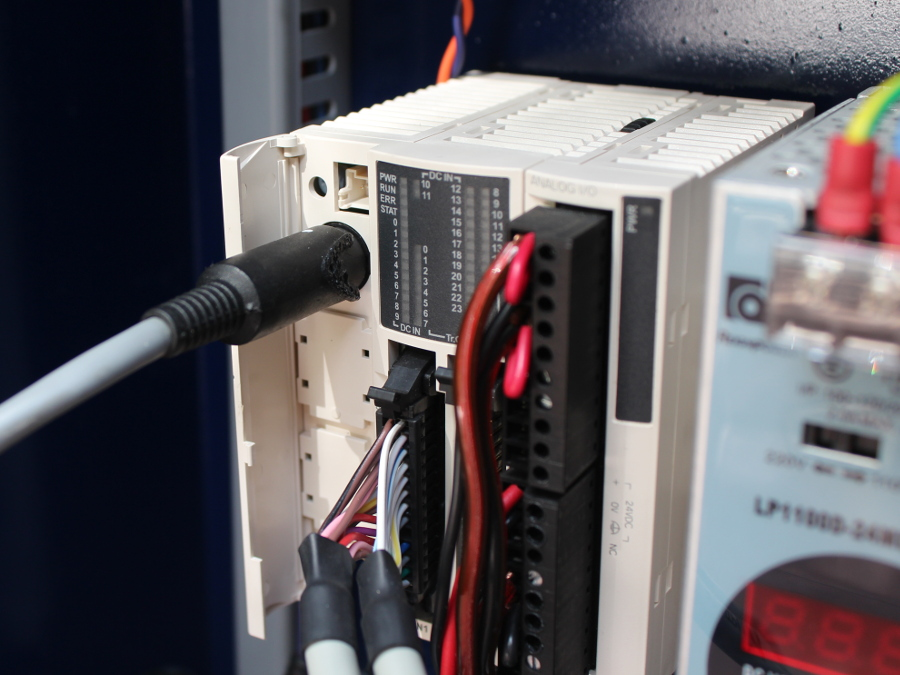
\includegraphics[width=\textwidth]{Sections/3-Tablero/Images/PLC.JPG}

			\footnotesize
			PLC Twido \texttt{40DTK}
			
			Módulo \texttt{AMM 6HT} ($4$-$20\,mA$ $12\,bits$)
			\end{center}
		\end{column}
	\end{columns}
}

\frame{
	\ifdebug
	\frametitle{Cableado de señal: Comunicación\hfill{\color{red}\emph{F}}}
	\else
	\frametitle{Cableado de señal: Comunicación}
	\fi

	
	PLC $\Rightarrow$ \texttt{RS485}
	
	Computador supervisor $\Rightarrow$ \texttt{RS232C}, \texttt{USB}
	\vspace{-.5cm}
	\begin{columns}[t]
	 \begin{column}{.5\textwidth}
	  \begin{center}
	   {\color{newcolor}Adaptador}
	  \end{center}
	  \vspace{-.25cm}
	\begin{itemize}
	 \item {\color{darkgreen1} Ventajas}
	 \begin{itemize}
	  \item Inmunidad a interferencias
	 \end{itemize}
	 \item {\color{newcolor3} Inconvenientes}
	 \begin{itemize}
	  \item Vínculo físico
	 \end{itemize}
	\end{itemize}
	\centering
	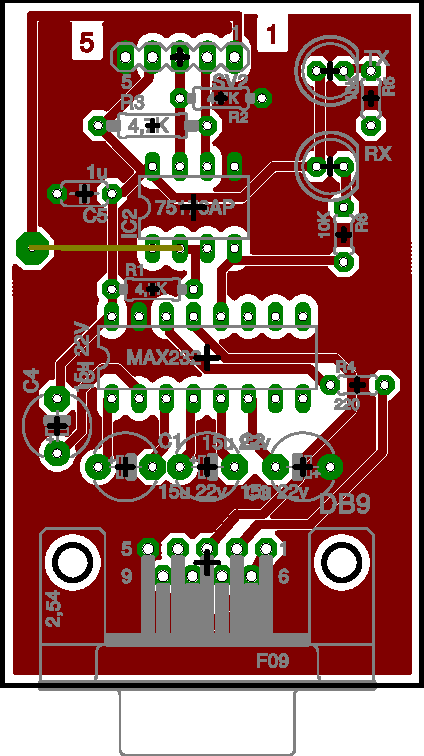
\includegraphics[height=3.9cm]
{Sections/3-Tablero/Images/Card.pdf}
	 \end{column}
	 \begin{column}{.5\textwidth}
	  \begin{center}
	  {\color{newcolor}Conexión inalámbrica}
	  \end{center}
	  \vspace{-.25cm}
	  \begin{itemize}
	 \item {\color{darkgreen1} Ventajas}
	 \begin{itemize}
	  \item Móvil
	 \end{itemize}
	 \item {\color{newcolor3} Inconvenientes}
	 \begin{itemize}
	  \item Alta latencia, timeouts
	 \end{itemize}

	\end{itemize}
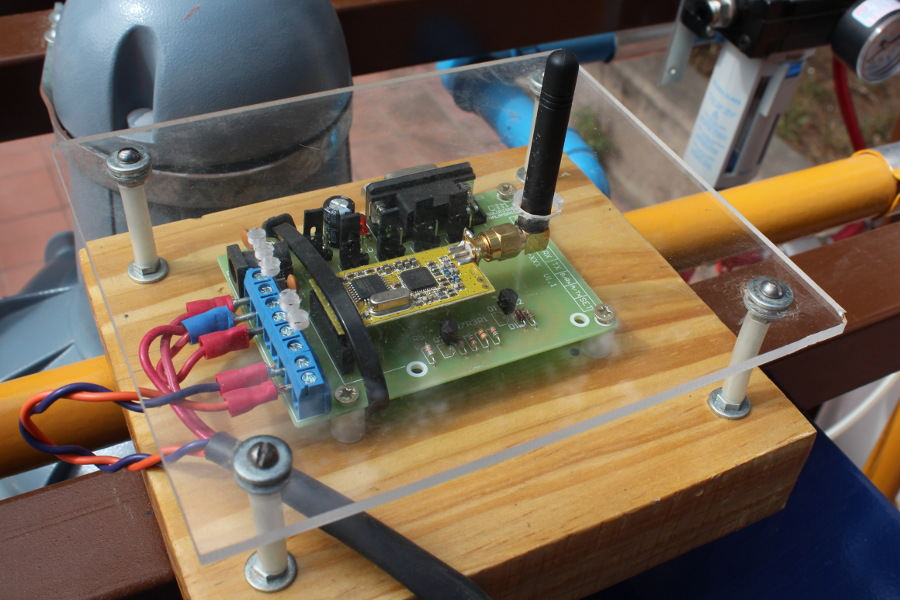
\includegraphics[width=\textwidth]
{Sections/3-Tablero/Images/IMG_5038.JPG}
	  
	 \end{column}
	\end{columns}
}